\documentclass[9pt,compress]{beamer}
\usepackage{amsmath}
\usepackage{url}
\usepackage{ucs}
\usepackage[utf8x]{inputenc}
\usepackage[ngerman]{babel}
\usepackage{ulem}  % sout
\usepackage{multicol}
\usepackage{setspace}
\usepackage{bookman}

\title{Newsflash}
\date{3. Oktober 2008}

\usetheme{Warsaw}  %Warsaw, Berkeley?
\usecolortheme{seahorse}
\usefonttheme{serif}
\useinnertheme{rectangles}
\setbeamercovered{transparent}

\begin{document}

\frame{
  \begin{center}
    \huge Einführung in die Welt der Microcontroller

    \vfill

    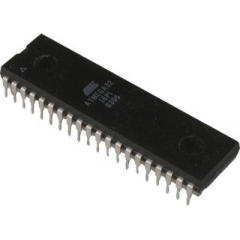
\includegraphics[scale=0.4]{atmega.jpg}
  \end{center}
}

\frame{
  \frametitle{Inhaltsverzeichnis}
    \tableofcontents
}

\section{Übersicht}
\subsection{Möglichkeiten}

\frame {

}

\frame {
  \frametitle{Was ist ein Microcontroller?}

  \begin{block}{Microcontroller}
    Ein Microcontroller ist ein Chip, der neben Prozessor und Arbeitsspeicher
    weitere Peripherie mitbringt.
  \end{block}

  \vfill

  Komponenten:
  \begin{itemize}
    \item Prozessor
    \item Arbeitsspeicher
    \item Flash-Speicher
    \item Eingabe-/Ausgabe
    \item Analog-/Digitalwandler
    \item EEPROM
    \item Timer/Counter
    \item Schnittstellen: UART, I2C (TWI), UART, USB\dots
  \end{itemize}
}

\frame {
  \frametitle{Wie schnell ist ein Mikrocontroller?}

  Eckdaten:

  \begin{itemize}
    \item Taktrate: bis 20MHz (8Bit)
    \item SRAM: bis 4kB
    \item FLASH: bis 128kB
    \item EEPROM: einige kB
  \end{itemize}

  \vfill
  \only<2-> { \huge LANGSAM?}
  \only<3-> { \vfill \large kommt drauf an, was man machen will\dots}
}

\subsection{Einsatz}
\frame {
  \frametitle{Wofür kann man einen Microcontroller einsetzen?}

  allgemein:
  \begin{itemize}
    \item Messen
    \item Steuern
    \item Kommunikation mit anderen Geräten (PCs/Microcontroller)
  \end{itemize}

  \vfill

  konkret (Beispiele):
  \begin{itemize}
    \item MP3-Player
    \item Lampe
    \item Alarmanlage
    \item Motorsteuerung
    \item Alkoholsensor
    \item USB-Geräte (Tastatur, Massenspeicher)
    \item Temperaturregler
    \item \dots
  \end{itemize}
}

\section{Microcontroller}

\frame {
  \frametitle{Atmega32}

  \begin{center}
    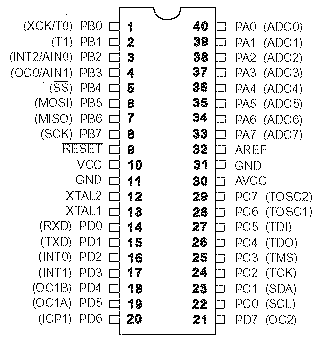
\includegraphics[scale=0.5]{atmega32.png}
  \end{center}
}

\subsection{Grundlegendes}

\frame {
  \frametitle{Prozessor}

  \begin{itemize}
    \item Herz des Microcontrollers
    \item beinhaltet Arithmetikfunktion, Stack Pointer, Register\dots
    \item RISC-Architektur; gute Optimierungsmöglichkeit für Compiler
    \item Unterscheidung anhand der Breite des internen Datenbusses: 4bit, 8bit, 16bit\dots
    \item Taktraten von 1MHz (intern) bis hin zu 16 MHz mit externem Quarz (z.B. Atmega32)
    \item 32 8-bit-breite Register; R26 bis R31 aber auch 3 16-bit breite Register
  \end{itemize}
}

\frame {
  \frametitle{Speicher und Register}

  Programmspeicher:
  \begin{itemize}
    \item Flash-Speicher mit dem Programm
    \item mind. 1.000-mal wieder beschreibbar
    \item Programm kann somit aktualisiert/erweitert/ersetzt werden
    \item ISP: MC kann innerhalb der Schaltung programmiert werden
  \end{itemize}

  \vfill

  Datenspeicher (SRAM):
  \begin{itemize}
    \item Speicher für temporäre Daten, die während der Laufzeit anfallen
    \item Unterscheidung von SRAM-Bereich und Registerbereich
    \item Registerbereich: Spiegelung der der Register, sowie Port-Zustände
    \item SRAM-Bereich: eigentlicher SRAM mit Stack
  \end{itemize}

  \vfill

  EEPROM:
  \begin{itemize}
    \item Daten bleiben stromlos erhalten
    \item 100.000 Schreib-/Löschzyklen
    \item ideal z.B. für Konfigurationsdateien
  \end{itemize}
}

\subsection{Peripherie}

\frame {
  \frametitle{Ports}

  \begin{itemize}
    \item Ports (und Peripherie im allgemeinen) erlaubt dem MC, mit der Außenwelt zu kommunizieren
    \item jeweils 8-Datenleitungen werden zu einem Port zusammengefasst
    \item Ports werden alphabetisch nummeriert: PORTA, PORTB, PORTC\dots
    \item Datenleitungen erlauben bidirektionale Kommunikation: senden und empfangen
    \item \textbf{vor} der Verwendung muss die Datenrichtung im Data-Direction-Register (DDR) angegeben werden
  \end{itemize}

  \vfill

  \begin{exampleblock}{Beispiel}
    DDRA  = 21; \ \ \ \  $\Rightarrow$ PA4, PA2, PA0 Ausgang, Rest Eingang\\
    PORTA = 3;  \ \ \ \  $\Rightarrow$ PA0, PA2 high, PA4 low
  \end{exampleblock}

}

\subsection{Interrupts}
\frame {
  \frametitle{Interrupts}

  \begin{block}{sequenzielle Abarbeitung von Befehlen}
    Microcontroller verarbeiten Befehle sequenziell, nicht parallel
  \end{block}

  \vfill

 Problem: schnelles Reagieren auf Ereignisse
 \begin{enumerate}
   \item \textbf{Pollen}:\\
   in einer Schleife Zustand überprüfen, bis er sich geändert hat
   \item \textbf{Interrupt}:\\
   tritt Ereignis ein, unterbricht der Prozessor seine Ausführung, merkt sich
   die Stelle, an der er gerade war, und führt eine Interrupt-Service-Routine
   aus
 \end{enumerate}
}

\subsection{ADC}
\frame {
  \frametitle{AD-Wandler}

  \begin{itemize}
    \item 10-Bit-ADC zum messen von Spannungen
    \item $2^{10}=1024 \Rightarrow$ 1024 unterschiedliche Spannungsstufen messbar
    \item Vergleich mit verschiedenen Spannungen
    \item Unterstützung von Interrupts
  \end{itemize}
}

\subsection{Timer}
\frame {
  \frametitle{Timer/Counter}

  \begin{itemize}
    \item Einheit, die eine Zahl mit einer speziellen Frequenz erhöht
    \item Unterstützung für interne und externe Zählfrequenz
    \item Atmega32: drei Timer/Counter mit 8-Bit und 16-Bit
    \item 10-Bit Prescaler
    \item Input Capture Unit (Zählen externer Ereignisse)
    \item CTC-Modus (Clear Timer on Compare Match)
    \item Unterstützung von PWM
  \end{itemize}

  \vfill

  \begin{center}
    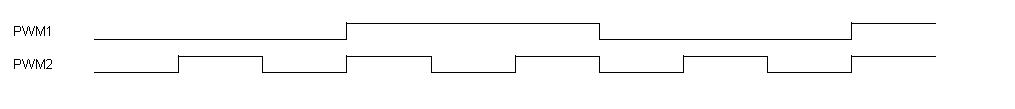
\includegraphics[scale=0.4]{pwm.JPG}
  \end{center}
}

\subsection{Rest}
\frame {
  \frametitle{Der Rest}

  \begin{itemize}
    \item Watchdog:\\automatischer Reset des Programms, falls es "hängt"

    \item I2C:\\
    serieller Zwei-Draht-Bus zur Datenübertragung
    \item SPI:\\
    serieller Datenbus zur Datenübertragung; wird für ISP verwendet
    \item UART:\\
    Senden und Empfangen von Daten
  \end{itemize}
}

\section{Schaltungen}
\subsection{Grundschaltungen für ATmega32}
\frame {
  \frametitle{Grundschaltung}

 \begin{center}
   \only<1> { 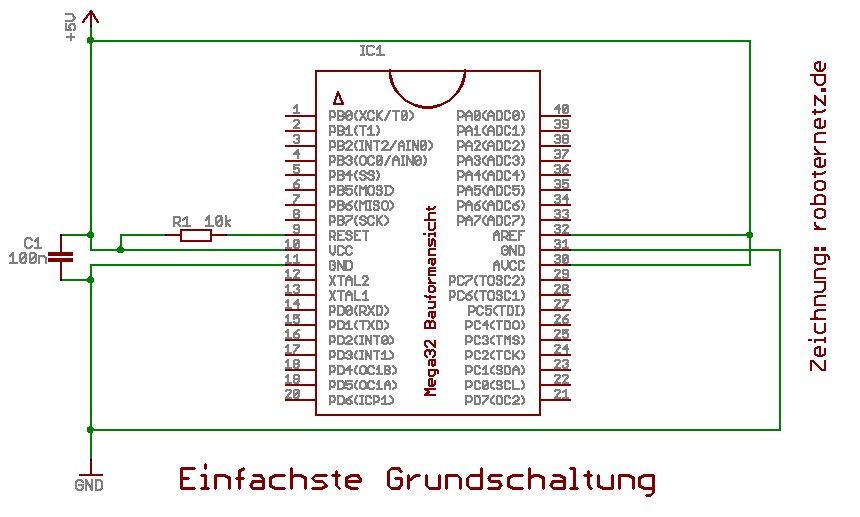
\includegraphics[scale=0.34]{s1.png} }
   \only<2> { 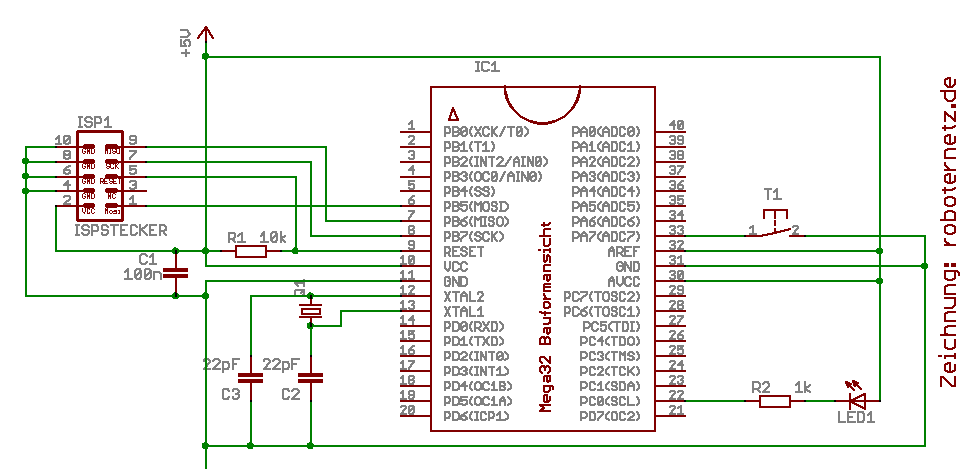
\includegraphics[scale=0.34]{s2.png} }
 \end{center}
}

\subsection{Stromversorgung}
\frame {
  \frametitle{Stromversorgung}

  \begin{center}
    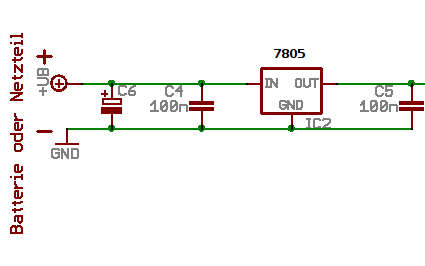
\includegraphics[scale=0.4]{spannung.png}
  \end{center}
}

\section{Sonstiges}
\subsection{Fuse-Bits, Sprachen, Programmer}
\frame {
  \frametitle{Dies und Das\dots}
  \begin{itemize}
    \item AVR-Fuses: Konfigurationsbits, die das Verhalten des Microcontrollers ändern:

    \begin{itemize}
      \item Fuse-Bit \textbf{setzen}: Wert  \textbf{0} schreiben
      \item Fuse-Bit \textbf{löschen}: Wert \textbf{1} schreiben
    \end{itemize}

    \item verwendete Programmiersprachen: Basic (Bascom), C (gcc-avr), Exoten wie Python\dots

    \item Programmer: usbprog, AVRISP MKII, Atmel AVR Dragon, parallel/seriell
    \item Liste von Programmern:\\ http://www.mikrocontroller.net/articles/AVR\_In\_System\_Programmer
  \end{itemize}
}

\frame {
  \huge Demo?
}

\subsection{Hilfe, weitere Informationen}
\frame {
  \frametitle{Hilfe/weitere Informationen}

  \begin{itemize}
    \item Mailingliste der Mikrocontroller Projektgruppe des ACF
    \item mikrocontroller.net: Forum, Codesammlung, Artikelsammlung
    \item roboternetz.de: Wissensbereich mit Wiki, Forum
    \item AVR-Risc — Embedded Software selbst entwickeln von Roman Mittermayr
  \end{itemize}
}

\end{document}
